\section{Block 1: Introduction}
We have simple 3-tier architecture which allows us to communicate with the server and extract data from our database. This protects the database from unwanted queries from the client.

\begin{center}
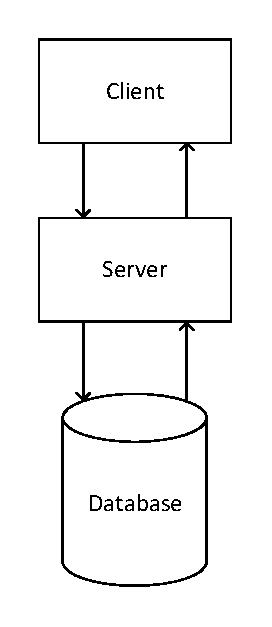
\includegraphics[scale=0.8]{3-tier.pdf}
\end{center}

\begin{enumerate}
\item The client opens his web browser and sends a HTTP request to the server.
\item The server runs the PHP script which queries data from the database.
\item The database returns the result according to the query.
\item Then the server returns the HTTP response to the client.
\item The response is then output as HTML.
\end{enumerate}

\begin{lstlisting}[language=php,label=lst:aspectratio] 
<?php
$connection = mysql_connect("localhost", "root", "");
mysql_select_db("webengi", $connection);

$query = mysql_query("SELECT testtext FROM hello", $connection);

while ($row = mysql_fetch_assoc($query)) {
    echo $row['testtext']."</br>";
}
?>
\end{lstlisting}

This code shows the steps explained above. We chose to run the server on localhost using WampServer, which also comes bundled with a MySQL database.

We start by connecting to the localhost with the username \textit{root} and empty password. Then we select the database called \textit{webengi}, and then query the database. For each row that is returned by the query, we echo the content of the column called \textit{testtext}.